%----------------------------------------------------------------------------------------------------------------------------------------------------------%
\chapter{Experimental design}
%----------------------------------------------------------------------------------------------------------------------------------------------------------%
\epigraph{It is common sense to take a method and try it; if it fails, admit it frankly and try another. But above all, try something.}{\textit{Anthony Burgess}}
%----------------------------------------------------------------------------------------------------------------------------------------------------------%
\paragraph{}This Extended Essay has the objective of studying bibliographically the effects of \emph{Staphylococcus aureus} on the human body, as well as the ways humanity has developed to defeat it. Experimentally, it has one main objective, and several secondary ones: mainly, I want to find out the natural prevalence of Staphylococcus Aureus among my fellow schoolmates. Secondarily, I want to improve my lab etiquette and fluidity; to improve my protocol-making, how I follow them in the lab and how I deal with problems that may arise from them; to learn how to work with limited resources; and to practice my staining and microscope use. The research question I will follow is 
\newline\begin{center}"\emph{What is the prevalence of \emph{Staphylococcus aureus} in our school}?"\end{center}
To which my hypothesis is \newline
\begin{center}\emph{``About 30\%``}.\end{center}\newline I would also like to know the answer to \newline
\begin{center}"\emph{Is the prevalence of \emph{Staphylococcus aureus} affected by gender or age?}"\end{center}
to which my hypothesis is \newline
\begin{center}\emph{``No``}.\end{center}
The variable I will study is the presence or not of the bacterium in question on different subjects, and compare it against their characteristics (such as approximate age and gender). I'll keep constant the culture medium, as well as the culture temperature and humidity.
%----------------------------------------------------------------------------------------------------------------------------------------------------------%
\section{Bill of materials}
\paragraph{}The materials used, as well as the quantities used, can be found in the following table. On the left, laboratory equipment and, on the right, reagents, staining agents, and consumables used:
\begin{center}\begin{figure}[H]\centering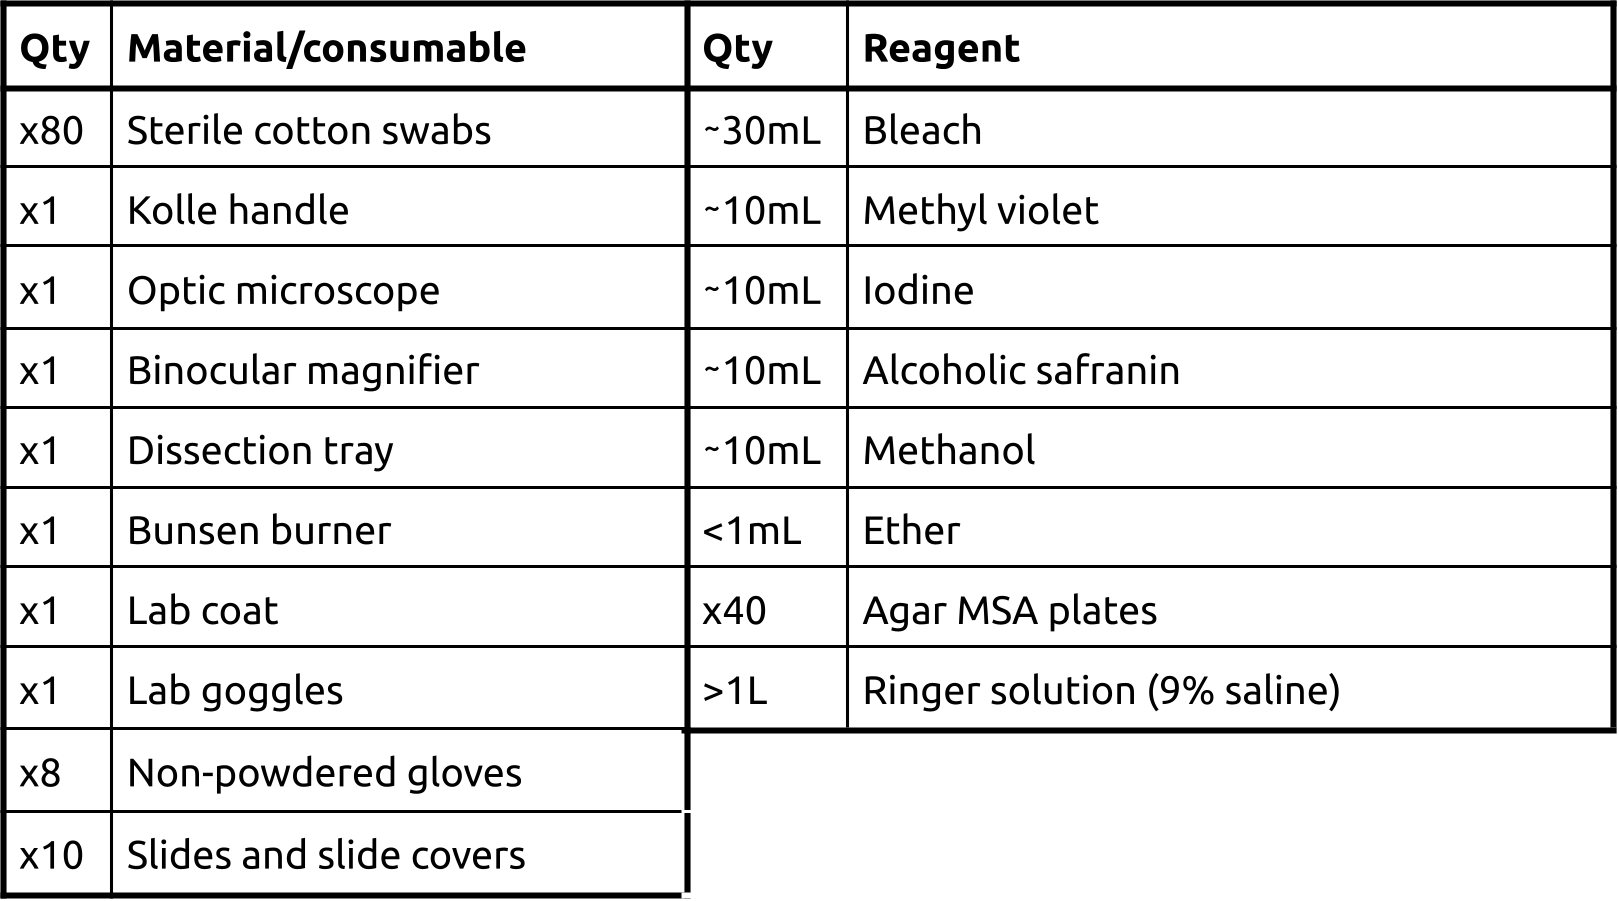
\includegraphics[width=0.90\textwidth]{BOM-1.png}\end{figure}\end{center}
%----------------------------------------------------------------------------------------------------------------------------------------------------------%
\section{Biosecurity and risk mitigation}
\paragraph{}Staph is considered a Biosecurity Level (BSL) 2 pathogenic bacteria\cite{cheungPathogenicityVirulenceStaphylococcus2021}. This means that it is associated with a human disease that can pose a moderate human health hazard. In a laboratory where BSL-2 pathogens are handled, usual lab rules should be followed (mechanical pipetting only, surgical hand-washing, prohibition of the consumption of food and drinks in the lab, proper PPE use… as well as avoiding splashes or aerosols, adhering biohazard warning signs present on all material used, as well as proper surface and material disinfection via the use of autoclave.\newline
The risks associated with this bacterium were assessed following the protocol designated by the World Health Organisation, and proper security measures were followed at all times when handling biohazardous material. No incidents occurred during the research\cite{worldhealthorganizationLaboratoryBiosafetyManual2020}.\newpage